	\documentclass{beamer}
	\usepackage[latin1]{inputenc}
	\usepackage{textpos}
	\usepackage{graphics}
	\usepackage[english]{babel}
	\usepackage{colortbl}
	\usepackage{caption}
	% \usepackage{subcaption}
	\usepackage{multirow}
	\usepackage{amsmath}
	\usepackage{xcolor} % for colored text

	\usepackage{tikz} % for flow charts
	\usetikzlibrary{shapes,arrows,positioning,shadows,calc}

\usepackage{filecontents}% http://ctan.org/pkg/filecontents
\usepackage{silence}% http://ctan.org/pkg/silence
\WarningFilter{latex}{Overwriting file}% Remove LaTeX warnings starting with "Overwriting file"
\begin{filecontents*}{linereg.data}
#x y
0 4
10 24
\end{filecontents*} 

\begin{filecontents*}{linereg2.data}
#x y
2 8
8 20
\end{filecontents*} 

	\renewcommand<>{\item}[1]{\only#2{\beameroriginal{\item}{#1}}} % for replace a equation for other equation in the same place
	
	% \usetheme{Warsaw}
	\usetheme{Frankfurt}
	% \usetheme{Boadilla}
	\setbeamertemplate{navigation symbols}{} 
	% \useoutertheme{infolines} 
\setbeamertemplate{footline}{\hbox{\vspace{0.1cm} \insertshortauthor \hspace*{3.0cm} \insertshorttitle \hspace*{4.0cm} \hfill\insertframenumber/\inserttotalframenumber}} 


\def\braces#1{[#1]} % to define square parenthesis 
	
% \usecolortheme{orchid}

% \usecolortheme{lily}

% \usecolortheme{default}
\usecolortheme{cranejavier}

% \setbeamertemplate{footline}[frame number]
% \setbeamertemplate{footline}[page number]
	
	
	% -------------------------------------- Slide 1
	\title[Landsat 8 over Case 2 Water]{The Use of Landsat 8 for Monitoring of Fresh and Coastal Water}
	\author[Javier A. Concha]{\Large Javier A. Concha \\\footnotesize Ph.D. Candidate\\ Advisor: Dr. John Schott}
	\institute{\footnotesize Digital Imaging and Remote Sensing Lab\\Chester F. Carlson Center for Imaging Science\\ Rochester Institute of Technology}
	\date{\today}
	
\begin{document}
{	
\setbeamertemplate{footline}{} 
\setbeamertemplate{headline}{}
	
	\begin{frame} 
	\titlepage
	
	\begin{textblock*}{10cm}(10.0cm,-8.5cm)
	   \includegraphics[height=10mm]{/Users/javier/Desktop/Javier/MASTER_RIT/2011_THESIS/LaTeX/Presentation/tiger_walking_rit_color.eps}
	\end{textblock*}
	\begin{textblock*}{10cm}(4.7cm,-8.0cm)
	   \includegraphics[height=5mm]{/Users/javier/Desktop/Javier/PHD_RIT/ConferencesAndApplications/2014_RITResearchSymposium/Images/USGS_logo.eps}
	\end{textblock*}	
	\begin{textblock*}{10cm}(-.7cm,-8.5cm)
	   \includegraphics[height=10mm]{/Users/javier/Desktop/Javier/PHD_RIT/ConferencesAndApplications/2014_ASPRS_SOY/Images/dirs_logo.png}
	\end{textblock*}
	
	\begin{textblock*}{9cm}(2cm,-5cm)

	   \tikz\node[opacity=0.3]{ \includegraphics[width=65mm]{/Users/javier/Desktop/Javier/PHD_RIT/ConferencesAndApplications/2014_ASPRS_SOY/Images/landsat8-earth.jpg}};
	\end{textblock*}

	\begin{textblock*}{12cm}(1cm,0cm)
	   \scriptsize Presented to: 2014 RIT Graduate Research and Creativity Symposium
	\end{textblock*}
	
	\end{frame}

}
\addtocounter{framenumber}{-1}
%\setbeamercovered{highly dynamic}
%\setbeamercovered{transparent}
\setbeamercovered{still covered={\opaqueness<1->{2}},again covered={\opaqueness<1->{2}}}

% ----------------------------------- Slide ----------------------------------------------	

\addtobeamertemplate{frametitle}{}{%
\begin{textblock*}{90mm}(8.2cm,-0.5cm)
% \includegraphics[height=0.5cm]{/Users/javier/Desktop/Javier/MASTER_RIT/SPIE2012/Slides/rit_white_no_bar.jpg}
\includegraphics[height=0.4cm]{/Users/javier/Desktop/Javier/PHD_RIT/ConferencesAndApplications/2014_ASPRS_SOY/Images/RIT_LOGO.png}
\end{textblock*}}


% ----------------------------------- Slide ----------------------------------------------
\begin{frame}{\LARGE Outline} 
	\tableofcontents
\end{frame}

\addtocounter{framenumber}{-1}

% \AtBeginSection[ ]
% {		
% 	\begin{frame}{\LARGE Outline} 
% 		\tableofcontents[currentsection]
% 	\end{frame}

% \addtocounter{framenumber}{-1}	
% }	

\AtBeginSubsection[ ]
{		
	\begin{frame}{\LARGE Outline} 
		\tableofcontents[currentsection,currentsubsection]
	\end{frame}
\addtocounter{framenumber}{-1}	
}	
%%%%%%%%%%%%%%%%%%%%%%%%%%%%%%%%%%%%%%%%%%%%%%%%%%%%%%%%%%%%%%%%%%%%%%%%%%%%%%%%%%%%%%%%%%
\section{Background}
% ------------------------------ SUBSECTION ----------------------------------------------
\subsection{Atmospheric Correction: ELM}
% ----------------------------------- Slide ----------------------------------------------
\begin{frame}{\LARGE Atmospheric Correction} 
 \begin{columns}[c] % contents are top vertically aligned
  	\begin{column}[T]{5cm} % each column can also be its own environment
    \includegraphics[height=5cm]{/Users/javier/Desktop/Javier/PHD_RIT/ConferencesAndApplications/2014_RITResearchSymposium/Images/SensorReachingRadiance.png}
    	    \vspace{0.2cm}
    		\centerline{Retrieve $L_w$}
     	\end{column}
  
  	\begin{column}[T]{7cm} % each column can also be its own environment
    \includegraphics[width=7cm]{/Users/javier/Desktop/Javier/PHD_RIT/ConferencesAndApplications/2014_RITResearchSymposium/Images/TOARadiance.png}
    	    \vspace{0.2cm}
    		\centerline{Retrieve $L_w$ vs $L_u$}
    		% \centerline{(Unknown concentrations)}
     	\end{column}
\end{columns}
\vspace{.5cm}
\hspace{4cm}{\scriptsize $*~$Images from: http://www.oceanopticsbook.info/}
\end{frame}
% ----------------------------------- Slide ----------------------------------------------
\begin{frame}{\LARGE Atmospheric Correction}
{\Large Empirical Line Method (ELM)} 
 \begin{columns}[c] % contents are top vertically aligned
  	\begin{column}[T]{5cm} % each column can also be its own environment
  	{\centering \Large $L(\lambda)=m\times r_d(\lambda)+b$}\\
  	\vspace{0.1cm}
  	where: \begin{tabbing} $L$: Radiance\\
  	$r_d$: Reflectance\\
  	$m$: slope\\
  	$b$: offset
  	\end{tabbing}
  	% \vspace{0.3cm}
    \begin{itemize}
    	\item Two pixels in the scene with known reflectance
    	\vspace{0.3cm}
    	\item Linear relationship between radiance $L$ and reflectance $r_d$ 	
    \end{itemize}
     	\end{column}
  
  	\begin{column}[T]{7cm} % each column can also be its own environment
	\centering
\begin{figure}[htb]
	\centering
\resizebox{7cm}{!}{%
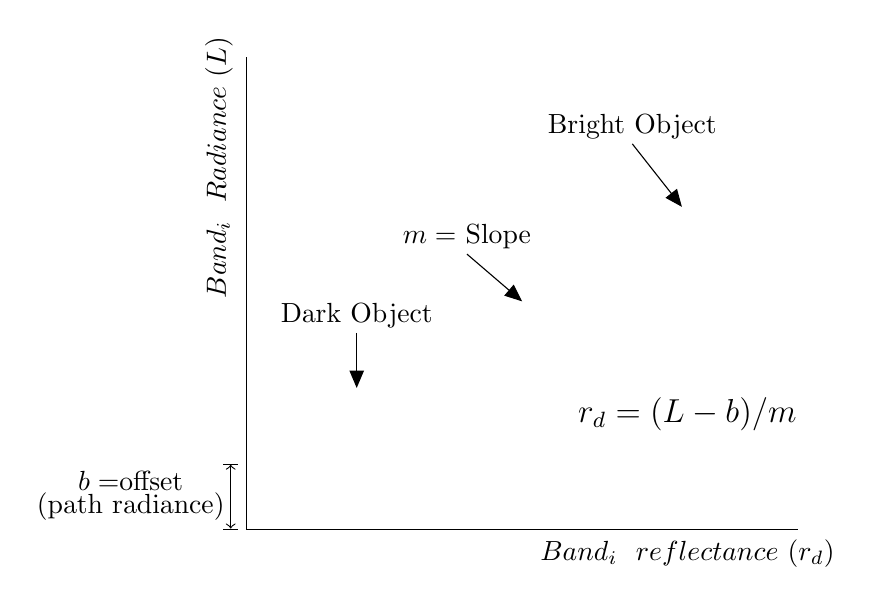
\begin{tikzpicture}[y=.2cm, x=.7cm]
 	%axis
	\draw (0,0) -- coordinate (x axis mid) (10,0);
    \draw (0,0) -- coordinate (y axis mid) (0,30);
    %ticks
 %  	\foreach \x in {0,...,10}
 %   		\draw (\x,1pt) -- (\x,-3pt)
	% node[anchor=north] {\x};
 %  	\foreach \y in {0,5,...,30}
 %   		\draw (1pt,\y) -- (-3pt,\y) 
 %   			node[anchor=east] {\y}; 
    %labels      
	\node[below=0ex] at (8,0) {$Band_i~~reflectance~(r_d)$};
	\node[rotate=90] at (-.5,23) {$Band_i~~Radiance~(L)$};

	\node[below=.2ex] at (-2.1,4.5) {$b=$offset};
	\node[below=1.4ex] at (-2.1,4.0) {(path radiance)};
	\draw[rotate=90,|<->|] (0,1) -- coordinate (x axis mid) (1.2,1);

	\node[below=0ex] at (2,15) {Dark Object};
	\draw[arrows=-triangle 45] (2,12.5) -- (2,9);

	\node[below=0ex] at (4,20) {$m=$ Slope};
	\draw[arrows=-triangle 45] (4,17.5) -- (5,14.5);

	\node[below=0ex] at (7,27) {Bright Object};
	\draw[arrows=-triangle 45] (7,24.5) -- (7.9,20.5);

	\node[below=0ex] at (8,9) {\large $r_d=(L-b)/m$};

	%plots
	\draw plot 
		file {linereg.data};
	\draw plot[mark=*] 
		file {linereg2.data};

\end{tikzpicture}
  }%close \resizebox
% \caption{Regression used in ELM to solve the linear relationship between reflectance $r_d$ and radiance $L$ using a dark and bright pixel from the scene. \label{fig:ELM}}
\end{figure}

     	\end{column}
\end{columns}

\end{frame}% ------------------------------ SUBSECTION ----------------------------------------------
\subsection{Landsat 8}
% ----------------------------------- Slide ----------------------------------------------
\begin{frame}{\LARGE Landsat 8 - OLI Specifications} 
\vspace{-.5cm}
\begin{itemize}
\LARGE
	\item Optical satellite (passive)
	\vspace{.2cm}
	\item Multispectral: 4 VIS, 1 NIR, 2 SWIR, 1 Pan
	\vspace{.2cm}
	\item Spatial resolution: 15/30/100m
	\vspace{.2cm}
	\item Temporal resolution: 16 days
	\vspace{.2cm}
	\item Bit depth: 12-bits quantization (4096 levels)
	\vspace{.2cm}
	\item Pushbroom satellite
\end{itemize}

\end{frame}
% % ----------------------------------- Slide ----------------------------------------------
% \begin{frame}{\LARGE Landsat 8} 

% \begin{figure}[H]
% 		\includegraphics[height=6cm]{/Users/javier/Desktop/Javier/PHD_RIT/ConferencesAndApplications/2014_ASPRS_SOY/Images/ldcmbands.png}
% \end{figure}

% \end{frame}
% ----------------------------------- Slide ----------------------------------------------
\begin{frame}{\LARGE Landsat 8 Image} 
\begin{figure}[htb]
  	\centering
  	\includegraphics[height=7cm]{/Users/javier/Desktop/Javier/PHD_RIT/Latex/Proposal/Images/LC80160302013262LGN00subset.jpg}
  % \caption{Portion of the Landsat 8 image to be corrected showing part of the Lake Ontario, nearby ponds and Downtown Rochester. \label{fig:Scene} } 
\end{figure}
\end{frame}
% ----------------------------------- Slide ----------------------------------------------
% ------------------------------ SUBSECTION ----------------------------------------------
\subsection{Physics Model: Hydrolight}
\begin{frame}{\LARGE Hydrolight} 
\centerline{\LARGE For the Dark Pixel and LUT generation}

\begin{figure}[H]
		\includegraphics[height=6cm]{/Users/javier/Desktop/Javier/PHD_RIT/ConferencesAndApplications/2014_ASPRS_SOY/Images/HLdiagram.pdf}
\end{figure}
\hspace{5cm}{$*~$IOPs: Inherent Optical Properties}
\end{frame}
%%%%%%%%%%%%%%%%%%%%%%%%%%%%%%%%%%%%%%%%%%%%%%%%%%%%%%%%%%%%%%%%%%%%%%%%%%%%%%%%%%%%%%%%%%
\section{Project}
% ----------------------------------- Slide ----------------------------------------------
% ------------------------------ SUBSECTION ----------------------------------------------
\subsection{Goal}
\begin{frame}{\LARGE Motivation} 
\vspace{-.5cm}
\begin{columns}[c] % contents are top vertically aligned
  	\begin{column}[T]{6cm} % each column can also be its own environment
  		\vspace{0.5cm}
      	\begin{itemize}
      	\Large
      		\item Ocean Color Satellites (e.g. MODIS, SeaWiFS): \\ \LARGE Global Studies
      	\end{itemize}
	\end{column}

  	\begin{column}[T]{6cm} % each column can also be its own environment
 		\begin{figure}[H]
 			\includegraphics[height=3cm]{/Users/javier/Desktop/Javier/PHD_RIT/ConferencesAndApplications/2014_ASPRS_SOY/Images/107325main_chloro_concentrate.jpg}
 		\end{figure}
 		\vspace{-0.7cm}
 		{\hspace{4.2cm}\tiny $*~$Credit: NASA}
 	\end{column}
\end{columns}

\begin{figure}[H]
		\includegraphics[height=4cm]{/Users/javier/Desktop/Javier/PHD_RIT/ConferencesAndApplications/2014_ASPRS_SOY/Images/DiffResol.png}
\end{figure}
\end{frame}
% ----------------------------------- Slide ----------------------------------------------
\begin{frame}{\LARGE Goal} 
\begin{itemize}
\LARGE

\item To Use Landsat 8 to retrieve Color Producing Agents (CPAs):
\begin{itemize}
	\Large
 	\item chlorophyll
 	\item colored dissolved organic matter (CDOM)
 	\item suspended minerals (SM or TSS)
 \end{itemize}
\vspace{.5cm}
\item Over Coastal and Inland Water (Case 2 Waters)
\vspace{.5cm}
\item Small/Medium Scale regions

\end{itemize}

\end{frame}


% ----------------------------------- Slide ----------------------------------------------
% ------------------------------ SUBSECTION ----------------------------------------------
\subsection{Retrieval Process}
\begin{frame}{\LARGE Retrieval Process} 

\begin{figure}[H]
		\includegraphics[height=6cm]{/Users/javier/Desktop/Javier/PHD_RIT/ConferencesAndApplications/2014_ASPRS_SOY/Images/RetProcess.pdf}
\end{figure}
\hspace{7.5cm}{\footnotesize $*~$LUT: Look-up table}
\end{frame}

% ----------------------------------- Slide ----------------------------------------------
\begin{frame}{\LARGE Atmospheric Correction} 
{\Large Model-Based ELM}

\begin{block}{\LARGE Bright Pixel}
 	\begin{itemize}
 	\Large
 		\item Radiance: PIF\footnotemark[1] from Landsat 8 image
 		\item Reflectance: PIF\footnotemark[1] from Landsat reflectance product
 	\end{itemize}
\end{block} 
% \vspace{0.1cm}
\begin{block}{\LARGE Dark Pixel}

	\begin{itemize}
	\Large
		\item Radiance: ROI\footnotemark[2] over water from Landsat 8 image
		\item Reflectance: Hydrolight
	\end{itemize}

\end{block}
\footnotetext[1]{Pseudo-Invariant Features}
\footnotetext[2]{Region of interest}

\end{frame}

% % ----------------------------------- Slide ----------------------------------------------
% \begin{frame}{\LARGE Pseudo-Invariant Features (PIFs)} 
% \begin{figure}[htb]
% 	\centering

% \resizebox{10cm}{!}{%	
%   \begin{tikzpicture}[node distance=0.75cm, auto]
%           \tikzset{
%                   basenode/.style={rectangle,rounded corners,draw=black,very thick, inner sep=1em, minimum size=3em, text centered,text width=2cm},
%                   productnode/.style={ellipse,rounded corners,draw=black, very thick, text centered,text width=1.5cm},
%                   myarrow/.style={->,>=stealth',thick, double = black},
%                   mylabel/.style={text width=7em, text centered}
%           }
%           % SWIR branch
%           \node[basenode] (SWIR) {SWIR 2\\ Band};
%           \node[basenode, below=of SWIR] (TS1) {Mask by Threshold (upward)};
%           \node[align=left, right=0.0 of TS1] (C1) {Urban\\Veget.\\Water};
%           \node[align=left, right=-0.15 of C1] (C2) {ON\\ON\\OFF};

%           % Ratio branch
%           \node[basenode, right=2.5cm of SWIR] (Ratio) {Ratio\\ NIR Band/ Red Band};
%           \node[basenode, below=of Ratio] (TS2) {Mask by Threshold (downward)};
%           \node[align=left, right=0.0 of TS2] (C3) {Urban\\Veget.\\Water};
%           \node[align=left, right=-0.15 of C3] (C4) {ON\\OFF\\ON};

%           % AND
%           \path (TS1.south)--(TS2.south) node[pos=.5,below=2cm] (AND) {.AND.};


%           % PIF Mask
%           \node[basenode, below=of AND] (PIFMask){PIF Mask};
%           \node[align=left, left=0.85 of PIFMask] (C5) {Urban\\Veget.\\Water};
%           \node[align=left, right=-0.15 of C5] (C6) {ON\\OFF\\OFF};

%           \node[basenode, below=of TS2,right=2.0cm of AND] (Image) {Image};
%           \path (Image.south)--(PIFMask.east) node[below=of Image,right=2cm of PIFMask] (AND2) {.AND.};
%           \node[basenode, right=2cm of AND2] (PIFIm){PIF Image};

%           \draw[myarrow] (SWIR)--(TS1);
%           \draw[myarrow] (Ratio)--(TS2);
%           \draw[myarrow] (TS1)--(AND);
%           \draw[myarrow] (TS2)--(AND);
%           \draw[myarrow] (AND)--(PIFMask);
%           \draw[myarrow] (Image)--(AND2);
%           \draw[myarrow] (PIFMask)--(AND2);
%           \draw[myarrow] (AND2)--(PIFIm);
%   \end{tikzpicture}
%   }%close \resizebox
% % \caption{Illustration of the logic used to segment PIF features. \label{fig:PIFflowchart}}
% \end{figure}
% \end{frame}
% ----------------------------------- Slide ----------------------------------------------
\begin{frame}{\LARGE Atmospheric Correction} 
{\Large Pseudo-Invariant Features -- Bright Pixel}

\begin{figure}[htb]
  \begin{minipage}[c]{0.48\linewidth}
    \centering
      \includegraphics[trim=30 0 30 0,clip,height=5cm]{/Users/javier/Desktop/Javier/PHD_RIT/Latex/Proposal/Images/DTROCL8falsecolor.jpg}  
    \vspace{0.3cm}
    \centerline{Downtown Rochester}
    \centerline{False Color Image}
  \end{minipage}
  \hfill
  \begin{minipage}[d]{0.48\linewidth}
    \centering
      \includegraphics[trim=30 0 30 0,clip,height=5cm]{/Users/javier/Desktop/Javier/PHD_RIT/Latex/Proposal/Images/PIFmaskApplied.jpg}
    \vspace{0.3cm}
    \centerline{Downtown Rochester}
    \centerline{PIF mask}
  \end{minipage}
  % \caption{PIF mask determination. (a) False color image, with vegetation in red and (b) PIF mask over downtown Rochester. \label{fig:PIFmask} } 
\end{figure}
\end{frame}

% % ----------------------------------- Slide ----------------------------------------------
% \begin{frame}{\LARGE Atmospheric Correction} 
% {\Large PIFs -- Bright Pixel}

% \begin{figure}[htb]
%   \begin{minipage}[c]{0.48\linewidth}
%     \centering
%       \includegraphics[height=4.8cm]{/Users/javier/Desktop/Javier/PHD_RIT/Latex/Proposal/Images/ZenithCorrection.eps}
%   % \caption{Mean values for nine scenes of the Landsat reflectance product after applying the master PIF mask. \label{fig:ZenithCorr} }   
%     \vspace{0.3cm}
%     \centerline{PIFs values for 9}
%     \centerline{Landsat reflectance images}
%   \end{minipage}
%   \hfill
%   \begin{minipage}[d]{0.48\linewidth}
%     \centering
%       \includegraphics[height=4.8cm]{/Users/javier/Desktop/Javier/PHD_RIT/Latex/Proposal/Images/ZenithCorrelation.eps}
%   % \caption{Linear regression between reflectance values and solar zenith angle for band 1 of the Landsat reflectance product. \label{fig:Band1Corr} }
%     \vspace{0.3cm}
%     \centerline{Band 1 - PIFs spectrum for 9}
%     \centerline{Landsat reflectance images}
%   \end{minipage}
%   % \caption{PIF mask determination. (a) False color image, with vegetation in red and (b) PIF mask over downtown Rochester. \label{fig:PIFmask} } 
% \end{figure}
% \end{frame}
% ----------------------------------- Slide ----------------------------------------------
\begin{frame}{\LARGE Atmospheric Correction} 
{\Large Dark Pixel}

\begin{columns}[c] % contents are top vertically aligned
  	\begin{column}[T]{6cm} % each column can also be its own environment

		\includegraphics[height=4cm]{/Users/javier/Desktop/Javier/PHD_RIT/ConferencesAndApplications/2014_RITResearchSymposium/Images/StudyArea.png}
	\end{column}

  	\begin{column}[T]{6cm} % each column can also be its own environment
  		\begin{itemize}
  			\item Radiance: Lake Ontario ROI
  			\vspace{.5cm}
  			\item Reflectance: Hydrolight with IOPs measured in the field over same ROI
  		\end{itemize}
 	\end{column}
\end{columns}

\end{frame}
% ----------------------------------- Slide ----------------------------------------------
\begin{frame}{\LARGE Atmospheric Correction} 
{\Large Model-Based ELM}
\centerline{\LARGE Bright and Dark Pixel}
\begin{figure}[htb]
  \centering
  \includegraphics[width=12cm]{/Users/javier/Desktop/Javier/PHD_RIT/Latex/Proposal/Images/ELMpixelsENVI.pdf}
  % \caption{Bright and Dark pixels used in ENVI to apply ELM. (a) Data spectra and (b) Field spectra \label{fig:ELMpxsENVI} } 
\end{figure}
\end{frame}
% ----------------------------------- Slide ----------------------------------------------
\begin{frame}{\LARGE Atmospheric Correction} 
{\Large Model-Based ELM -- Results}
\vspace{-.5cm}
\begin{figure}[htb]
\centering
\includegraphics[height=6cm]{./Images/ELMcomparison.eps}
      
\end{figure}
\centerline{Comparison between traditional ELM (dashed lines)}
\centerline{and model-based ELM (solid lines).}
\end{frame}
% ----------------------------------- Slide ----------------------------------------------
\begin{frame}{\LARGE Retrieval Process} 

\begin{figure}[H]
		\includegraphics[height=7cm]{/Users/javier/Desktop/Javier/PHD_RIT/ConferencesAndApplications/2014_ASPRS_SOY/Images/RetProcess.pdf}
\end{figure}

\end{frame}
% ----------------------------------- Slide ----------------------------------------------

\begin{frame}{\LARGE Retrieval} 
{\vspace{0.1cm} \Large LUT from Hydrolight}
% \begin{block}{\footnotesize LUT}
  \begin{columns}[c] % contents are top vertically aligned
  	\begin{column}[T]{6cm} % each column can also be its own environment
  	\vspace{0.2cm}
    	\includegraphics[height=5cm]{/Users/javier/Desktop/Javier/PHD_RIT/ConferencesAndApplications/2014_ASPRS_SOY/Images/LUT.eps}
    	    \vspace{0.2cm}
    		\centerline{LUT}
    		\centerline{(Known concentrations)}
    \end{column}
  	\hspace{.3cm}
  	\begin{column}[T]{6cm} % each column can also be its own environment
  	\vspace{0.2cm}
	\scriptsize \addtolength{\tabcolsep}{-5pt}
		\begin{tabular}{c|c|c|c}
        		\bfseries{$<CHL>$}  	& \bfseries{$<SM>$}  & \bfseries{$a_{CDOM}(440)$} & \bfseries{$Backscatter$} \\
		$[ug/L]$  		& $[mg/L]$ & 	$[1/m]$ &	\bfseries{$Fraction$}, $[\%]$	\\ \hline \hline
0.1   & 1.0  &  0.11 &  0.5 \\
0.5   & 2.0  &  0.15 &  1.0 \\
1.0   & 5.0  &  0.21 &  1.5 \\
3.0   & 10.0 &  0.6  &  2.0 \\
10.0  & 25.0 &  1.0  &  --  \\
20.0  & 45.0 &  1.2  &  --  \\
40.0  & 50.0 &  --   &  --  \\
60.0  & --   &  --   &  --  \\  
90.0  & --   &  --   &  --  \\  
110.0 & --   &  --   &  --  \\  
135.0 & --   &  --   &  --  \\  
150.0 & --   &  --   &  --  \\     
	 	\end{tabular}
     	\end{column}
\end{columns}
% \end{block}
\end{frame}
% ----------------------------------- Slide ----------------------------------------------
\begin{frame}{\LARGE Retrieval} 
{\vspace{0.1cm} \Large LUT and Water Pixels}
 \begin{columns}[c] % contents are top vertically aligned
  	\begin{column}[T]{6.5cm} % each column can also be its own environment
    \includegraphics[height=5cm]{/Users/javier/Desktop/Javier/PHD_RIT/ConferencesAndApplications/2014_ASPRS_SOY/Images/LUT.eps}
    	    \vspace{0.2cm}
    		\centerline{LUT}
    		\centerline{(Known concentrations)}
     	\end{column}
  
  	\begin{column}[T]{6.5cm} % each column can also be its own environment
    \includegraphics[height=5cm]{/Users/javier/Desktop/Javier/PHD_RIT/ConferencesAndApplications/2014_ASPRS_SOY/Images/waterpixels.eps}
    	    \vspace{0.2cm}
    		\centerline{Water Pixels}
    		\centerline{(Unknown concentrations)}
     	\end{column}
\end{columns}
\end{frame}
% ----------------------------------- Slide ----------------------------------------------
\begin{frame}{\LARGE Retrieval} 
{\vspace{0.1cm} \Large Preliminary Results}

\begin{figure}[htb]
\centering
\includegraphics[height=6cm]{/Users/javier/Desktop/Javier/PHD_RIT/ConferencesAndApplications/2014_RITResearchSymposium/Images/RetrievalResults.eps}
      
\end{figure}
% \centerline{Comparison between traditional ELM (dashed lines)}
% \centerline{and model-based ELM (solid lines).}
\end{frame}
% ----------------------------------- Slide ----------------------------------------------
% ------------------------------ SUBSECTION ----------------------------------------------
\subsection{Field Collection and Lab Measurements}
\begin{frame}{\LARGE Field Collection} 
\begin{figure}[htb]
  \centering
  \includegraphics[width=8cm]{/Users/javier/Desktop/Javier/PHD_RIT/Latex/Proposal/Images/groundtruth-sitenames-no-ends.jpg}
  % \caption{Sites in the Rochester Embayment for the water sample collection on September, $19^{th}$, 2013.\label{fig:0910913Sites} } 
\end{figure}
\end{frame}
% ----------------------------------- Slide ----------------------------------------------
\begin{frame}{\LARGE Field Collection (con't)} 
\vspace{-1cm}
\begin{figure}[htb]
\centering
\includegraphics[height=7cm]{/Users/javier/Desktop/Javier/PHD_RIT/ConferencesAndApplications/2014_ASPRS_SOY/Images/Collection.pdf}
      
\end{figure}
% \centerline{Comparison between traditional ELM (dashed lines)}
% \centerline{and model-based ELM (solid lines).}
\end{frame}
% ----------------------------------- Slide ----------------------------------------------
\begin{frame}{\LARGE Lab Measurements} 
\vspace{-1cm}
\begin{figure}[htb]
\centering
\includegraphics[height=7cm]{/Users/javier/Desktop/Javier/PHD_RIT/ConferencesAndApplications/2014_ASPRS_SOY/Images/LabMeasurements.pdf}
      
\end{figure}
% \centerline{Comparison between traditional ELM (dashed lines)}
% \centerline{and model-based ELM (solid lines).}
\end{frame}
%%%%%%%%%%%%%%%%%%%%%%%%%%%%%%%%%%%%%%%%%%%%%%%%%%%%%%%%%%%%%%%%%%%%%%%%%%%%%%%%%%%%%%%%%%
\section{Future Work and Take Home Points}
% ------------------------------ SUBSECTION ----------------------------------------------
\subsection{}
\begin{frame}{\LARGE Outline} 
	\tableofcontents[currentsection]
\end{frame}
\addtocounter{framenumber}{-1}
% ----------------------------------- Slide ----------------------------------------------
\begin{frame}{\LARGE Future Work} 
\begin{itemize}
\Large
\setbeamercovered{transparent}
    \uncover<2->{
	\item Enhancement of atmospheric correction and retrieval process}
	\vspace{.5cm}
	\uncover<3->{
	\item Include a glint correction}
	\vspace{.5cm}
	\uncover<4->{
	\item To try retrieval in a different water body}
	\vspace{.5cm}
	\uncover<5->{
	\item Validation by comparing with products from ocean color satellites}
	\vspace{.5cm}
	\uncover<6->{
	\item Integration with Hydrodynamics models}
\end{itemize}
\end{frame}
% ----------------------------------- Slide ----------------------------------------------
\begin{frame}{\LARGE Take Home Points} 
\begin{itemize}
\Large
\setbeamercovered{transparent}
    \uncover<2->{
	\item Landsat 8 has a great potential to help in fresh and coastal water quality studies}
	\vspace{\baselineskip}
	\uncover<3->{
	\item Atmospheric correction over water is an essential step}
	\vspace{\baselineskip}
	\uncover<4->{
	\item Hydrolight is an excellent tool BUT needs specific water characteristics}
\end{itemize}
\end{frame}
 % ----------------------------------- Slide ----------------------------------------------
% \section*{}
% \begin{frame}%[shrink=30] 
% \tiny
%   \frametitle{References}
%   \nocite{*}
%   \bibliographystyle{apalike}
%   \bibliography{HLbeamerbib}
% \end{frame}

%% ----------------------------------- Slide ----------------------------------------------

{	
\setbeamertemplate{footline}{} 
\setbeamertemplate{headline}{}
\begin{frame}[noframenumbering] 

\vspace{\baselineskip}
\centerline{\Large Thanks for your attention!}
	\vspace{\baselineskip}

% \centerline{\Huge QUESTIONS?}
\uncover <2->{\centerline{\Huge QUESTIONS?}}
\vspace{\baselineskip}
\centerline{Javier A. Concha}
\centerline{jxc4005@rit.edu}

\begin{figure}[htb]
\centering
\includegraphics[height=5cm]{/Users/javier/Desktop/Javier/PHD_RIT/ConferencesAndApplications/2014_ASPRS_SOY/Images/LC80160302013262LGN00.jpg}
\end{figure}

\end{frame}
}

% ----------------------------------- Slide ----------------------------------------------
\end{document} % EEEEEEEEEEENNNNNNNNNNNNNNDDDDDDDDDDDD